% Created 2022-09-14 mié 10:37
% Intended LaTeX compiler: pdflatex
\documentclass[aspectratio=169, usenames,svgnames,dvipsnames]{beamer}
\usepackage[utf8]{inputenc}
\usepackage[T1]{fontenc}
\usepackage{graphicx}
\usepackage{grffile}
\usepackage{longtable}
\usepackage{wrapfig}
\usepackage{rotating}
\usepackage[normalem]{ulem}
\usepackage{amsmath}
\usepackage{textcomp}
\usepackage{amssymb}
\usepackage{capt-of}
\usepackage{hyperref}
\usepackage{color}
\usepackage{listings}
\usepackage{mathpazo}
\usepackage{gensymb}
\usepackage{amsmath}
\usepackage{diffcoeff}
\usepackage{steinmetz}
\usepackage{mathtools}
\bibliographystyle{plain}
\usepackage{siunitx}
\sisetup{output-decimal-marker={,}}
\DeclareSIUnit{\watthour}{Wh}
\hypersetup{colorlinks=true, linkcolor=Blue, urlcolor=Blue}
\renewcommand{\thefootnote}{\fnsymbol{footnote}}
\newcommand{\laplace}[1]{\mathbf{#1}(\mathbf{s})}
\newcommand{\slp}{\mathbf{s}}
\newcommand{\fasor}[1]{\mathbf{#1}(\omega)}
\newcommand{\atan}{\mathrm{atan}}
\parskip=5pt
\usetheme{Boadilla}
\usecolortheme{rose}
\usefonttheme{serif}
\author{Oscar Perpiñán Lamigueiro}
\date{}
\title{Respuesta en Frecuencia: Resonancia}
\subtitle{Teoría de Circuitos III}
\setbeamercolor{alerted text}{fg=blue!50!black} \setbeamerfont{alerted text}{series=\bfseries}
\AtBeginSubsection[]{\begin{frame}[plain]\tableofcontents[currentsubsection,sectionstyle=show/shaded,subsectionstyle=show/shaded/hide]\end{frame}}
\AtBeginSection[]{\begin{frame}[plain]\tableofcontents[currentsection,hideallsubsections]\end{frame}}
\beamertemplatenavigationsymbolsempty
\setbeamertemplate{footline}[frame number]
\setbeamertemplate{itemize items}[triangle]
\setbeamertemplate{enumerate items}[circle]
\setbeamertemplate{section in toc}[circle]
\setbeamertemplate{subsection in toc}[circle]
\hypersetup{
 pdfauthor={Oscar Perpiñán Lamigueiro},
 pdftitle={Respuesta en Frecuencia: Resonancia},
 pdfkeywords={},
 pdfsubject={},
 pdfcreator={Emacs 27.1 (Org mode 9.4.6)}, 
 pdflang={Spanish}}
\begin{document}

\maketitle

\section{Definiciones}
\label{sec:org2333f3c}
\begin{frame}[label={sec:orged7f565}]{Definición}
\begin{itemize}
\item Cuando un circuito eléctrico está en resonancia:
\begin{itemize}
\item La \alert{parte imaginaria} de su impedancia/admitancia es \alert{nula}.
\item La \alert{tensión y corriente} están en \alert{fase}.
\item La \alert{potencia reactiva} neta es \alert{nula}.
\end{itemize}
\item La resonancia se produce en una \alert{frecuencia determinada}, \(f_0\).
\item Sólo puede ocurrir en circuitos con \alert{al menos un inductor y un capacitor}.
\end{itemize}
\end{frame}

\begin{frame}[label={sec:org7f4f6dd}]{Ancho de Banda y Factor de Calidad}
\begin{columns}
\begin{column}{0.5\columnwidth}
\begin{itemize}
\item Frecuencias de potencia mitad: \(\omega_1, \omega_2\)
\end{itemize}
\begin{align*}
  |\fasor{Z}|_{\omega = \omega_{1,2}} &=  \frac{1}{\sqrt{2}}\cdot |\mathbf{Z}(\omega_0)|\\
  |\fasor{Y}|_{\omega = \omega_{1,2}} &=  \frac{1}{\sqrt{2}}\cdot |\mathbf{Y}(\omega_0)|
\end{align*}
\end{column}
\begin{column}{0.5\columnwidth}
\begin{center}
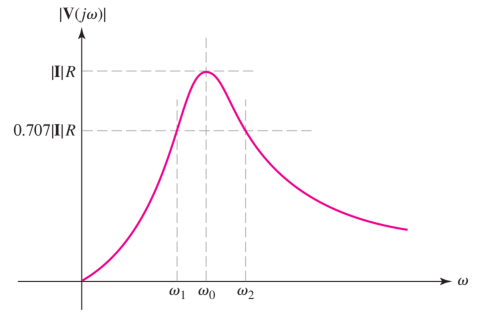
\includegraphics[width=.9\linewidth]{../figs/CurvaResonancia.pdf}
\end{center}
\end{column}
\end{columns}

\begin{itemize}
\item Ancho de Banda (\emph{de potencia mitad}):
\end{itemize}
\[
  B = \omega_2 - \omega_1
\]

\begin{itemize}
\item Factor de Calidad (\emph{en resonancia}):
\end{itemize}
\[
  \boxed{Q_0 = \frac{\omega_0}{B}}
\]
\end{frame}

\begin{frame}[label={sec:org64f1c63}]{Ancho de Banda y Factor de Calidad}
\begin{center}
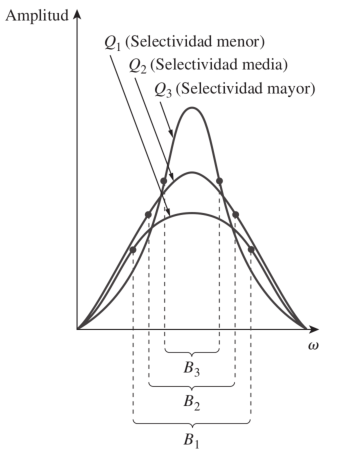
\includegraphics[height=0.9\textheight]{../figs/Q_B.pdf}
\end{center}
\end{frame}
\section{Circuito RLC paralelo}
\label{sec:orgd15fc86}


\begin{frame}[label={sec:org936a5fe}]{Admitancia}
\begin{center}
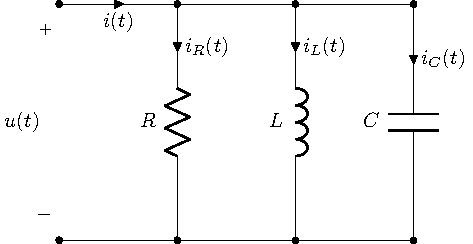
\includegraphics[height=0.25\textheight]{../figs/RLC_paralelo_resonante.pdf}
\end{center}

\begin{itemize}
\item Admitancia:
\end{itemize}
\[
  \fasor{Y} = \frac{1}{R} + j(\omega C - \frac{1}{\omega L})
\]
\begin{itemize}
\item Módulo en resonancia \(\omega_0\):
\end{itemize}
\[
  |\mathbf{Y}(\omega_0)| = \frac{1}{R} \rightarrow \omega_0 C - \frac{1}{\omega_0 L} = 0
\]

\[
  \boxed{\omega_0 = \frac{1}{\sqrt{LC}}}
\]
\end{frame}

\begin{frame}[label={sec:orgc0d5193}]{Puntos de Potencia Mitad}
\begin{itemize}
\item Definición de Puntos de potencia mitad (\(\omega_1, \omega_2\))
\end{itemize}
\begin{align*}
|\mathbf{Y}(\omega_1)| &= \frac{1}{\sqrt{2} R} \xrightarrow{\textcolor{blue}{\omega_1 < \omega_0}} \omega_1 C - \frac{1}{\omega_1 L} = \textcolor{blue}{-}\frac{1}{R}\\
|\mathbf{Y}(\omega_2)| &= \frac{1}{\sqrt{2} R} \xrightarrow{\textcolor{blue}{\omega_2 > \omega_0}} \omega_2 C - \frac{1}{\omega_2 L} =  \textcolor{blue}{+}\frac{1}{R}
\end{align*}

\begin{itemize}
\item Ecuaciones
\end{itemize}
\begin{align*}
  \omega_1^2 \omega_0^2 \textcolor{blue}{+} \frac{\omega_1 L}{R} - 1 &= 0\\
  \omega_2^2 \omega_0^2 \textcolor{blue}{-} \frac{\omega_2 L}{R} - 1 &= 0
\end{align*}
\end{frame}

\begin{frame}[label={sec:org15e3c13}]{Ancho de Banda y Factor de Calidad}
\begin{itemize}
\item Resultado
\end{itemize}
\begin{align*}
\omega_1 &= \textcolor{blue}{-}\frac{1}{2RC} + \sqrt{\left(\frac{1}{2RC}\right)^2 + \frac{1}{LC}}\\
\omega_2 &= \textcolor{blue}{+}\frac{1}{2RC} + \sqrt{\left(\frac{1}{2RC}\right)^2 + \frac{1}{LC}}
\end{align*}

\begin{itemize}
\item Ancho de Banda
\end{itemize}
\[
\boxed{B = \omega_2 - \omega_1 = \frac{1}{RC}}
\]

\begin{itemize}
\item Factor de Calidad
\end{itemize}
\[
  \boxed{Q_0 = \frac{\omega_0}{B} = \omega_0 R C = \frac{R}{\omega_0 L}}
\]
\end{frame}

\begin{frame}[label={sec:org3678229}]{Balance de corrientes en resonancia}
\begin{center}
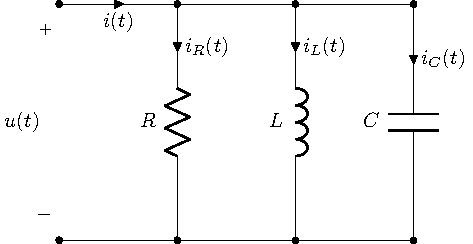
\includegraphics[height=0.35\textheight]{../figs/RLC_paralelo_resonante.pdf}
\end{center}

\[
  u(t) = U_0 \sin(\omega_0 t)
\]

\[
\left.
\begin{array}{l}
  i_R(t) = \frac{U_0}{R} \sin(\omega_0 t)\\
  i_L(t) = - \frac{U_0}{\omega_0 L} \cos(\omega_0 t)\\
  i_C(t) = \omega_0 C U_0 \cos(\omega_0 t)
\end{array}
\right\} \xrightarrow{\omega_0 = \frac{1}{\sqrt{LC}}} \boxed{i(t) = i_R(t)}
\]
\end{frame}

\begin{frame}[label={sec:orgc76c8a0}]{Balance de corrientes en resonancia}
\begin{center}
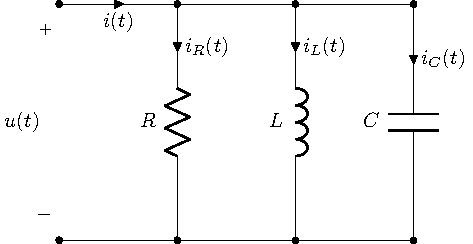
\includegraphics[height=0.25\textheight]{../figs/RLC_paralelo_resonante.pdf}
\end{center}

\begin{itemize}
\item Valores máximos (\alert{atención en circuitos con \(Q\) alto})
\end{itemize}
\[
  I_{R0} = \max\{i_R(t)\} = \frac{U_0}{R}
\]

\[
  I_{L0} = \max\{i_L(t)\} = \frac{U_0}{\omega_0 L} \xrightarrow{Q_0 = \frac{R}{\omega_0L}} \boxed{\frac{I_{L0}}{I_{R0}} = Q_0}
\]

\[
  I_{C0} = \max\{i_C(t)\} = \omega_0 C U_0 \xrightarrow{Q_0 = \omega_0CR} \boxed{\frac{I_{C0}}{I_{R0}} = Q_0}
\]
\end{frame}

\begin{frame}[label={sec:orga7c5aff}]{Balance de Energías}
\[
  u(t) = U_0 \sin(\omega t)
\]

\begin{itemize}
\item Energías total almacenada en \(\omega \neq \omega_0\):
\end{itemize}
\begin{align*}
  w_L(t) &= \frac{1}{2} L i_L^2(t) = \frac{U_0^2}{2 \omega^2 L} \cos^2 (\omega t)\\
  w_C(t) &= \frac{1}{2} C u^2(t) = \frac{U_0^2 C}{2} \sin^2 (\omega t) \\
  \cline{1-2}
  w_C(t) + w_L(t) &= \frac{U_0^2}{2} \left(C\sin^2(\omega t) + \frac{U_0^2}{2 \omega^2 L} \cos^2(\omega t)\right)
\end{align*}

\begin{itemize}
\item La energía almacenada en resonancia es \alert{constante}:
\end{itemize}
\[
\omega = \omega_0 = \frac{1}{\sqrt{LC}} \rightarrow \boxed{w_C(t) + w_L(t) = \frac{1}{2} C U_0^2}
\]
\end{frame}

\begin{frame}[label={sec:org4b578be}]{Nueva definición del Factor de Calidad}
\begin{itemize}
\item Energía almacenada en resonancia:
\end{itemize}
\[
w_{total} = \frac{1}{2} C U_0^2 = C U^2
\]

\begin{itemize}
\item Energía disipada en un período
\end{itemize}
\[
P_R = \frac{U^2}{R} \rightarrow w_R = T_0 \cdot \frac{U^2}{R}
\]

\begin{itemize}
\item Ratio entre almacenamiento y disipación
\end{itemize}

\[
\frac{w_{total}}{w_R} = f_0 C R \xrightarrow{Q_0 = \omega_0 C R} \boxed{Q_0 = 2 \pi \frac{w_{total}}{w_R}}
\]

\begin{itemize}
\item Un circuito resonante almacena \(Q_0/2\pi\) veces la energía suministrada.
\end{itemize}
\end{frame}

\begin{frame}[label={sec:orgce83d6f}]{La curva de resonancia \alert{no} es simétrica}
La frecuencia de resonancia no está en el centro del ancho de banda
\begin{center}
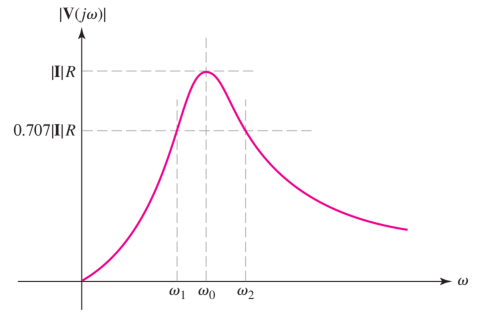
\includegraphics[height=0.6\textheight]{../figs/CurvaResonancia.pdf}
\end{center}
\end{frame}

\begin{frame}[label={sec:org95a7af0}]{La curva de resonancia \alert{no} es simétrica}
\begin{itemize}
\item Retomamos expresión de puntos de potencia mitad:
\end{itemize}
\[
\omega_{1,2} = \sqrt{\left(\frac{1}{2RC}\right)^2 + \frac{1}{LC}} \mp \frac{1}{2RC}
\]

\begin{itemize}
\item Los expresamos en función de \(Q\) y \(\omega_0\):
\end{itemize}

\[
\omega_{1,2}= \omega_0\left(\sqrt{\left(\frac{1}{2Q_0}\right)^2 + 1} \mp \frac{1}{2Q_0}\right)
\]

\begin{itemize}
\item La frecuencia de resonancia es la media geométrica (\emph{no está en el centro del ancho de banda}).
\end{itemize}
\[
  \boxed{\omega_1 \cdot \omega_2 = \omega_0^2} 
\]
\end{frame}

\begin{frame}[label={sec:orgc0ae54e}]{Aproximación para circuitos con alto \(Q_0\)}
\begin{itemize}
\item Cuando \(Q \geq 10\) podemos escribir:
\end{itemize}
\begin{align*}
\omega_1 &\simeq \omega_0\left(1 - \frac{1}{2Q_0}\right) = \omega_0 - \frac{B}{2}\\
\omega_2 &\simeq \omega_0\left(1 + \frac{1}{2Q_0}\right) = \omega_0 + \frac{B}{2}
\end{align*}

\begin{itemize}
\item En circuitos de \alert{alto factor de calidad}, la frecuencia de resonancia está \alert{aproximadamente} en el \alert{centro} del ancho de banda.
\end{itemize}

\[
  \boxed{\omega_0 \simeq \frac{1}{2}(\omega_1 + \omega2)}
\]
\end{frame}

\begin{frame}[label={sec:org9c0e4be}]{Admitancia en función de \(\omega_0\) y \(Q_0\)}
\begin{itemize}
\item Recordamos expresión de la admitancia:
\end{itemize}

\[
  \fasor{Y} = \frac{1}{R} + j(\omega C - \frac{1}{\omega L})
\]
\begin{itemize}
\item Expresamos los componentes en función de \(Q\) y \(\omega_0\):
\end{itemize}
\begin{align*}
  Q_0 = \omega_0 C R &\rightarrow C = \frac{Q_0}{\omega_0 R}\\
  Q_0 = \frac{R}{\omega_0 L} &\rightarrow \frac{1}{L} = \frac{\omega_0 Q_0}{R}
\end{align*}

\begin{itemize}
\item Admitancia expresada en función de \(Q_0\) y \(\omega_0\):
\end{itemize}
\[
  \boxed{\fasor{Y} = \frac{1}{R} \left[1 + j Q_0 \left(\frac{\omega}{\omega_0} - \frac{\omega_0}{\omega}\right)\right]} \rightarrow \mathbf{Y}(\omega_0) = \frac{1}{R} = Y_0
\]
\end{frame}

\begin{frame}[label={sec:org26dcfe9}]{Desintonización Relativa}
\begin{itemize}
\item Definimos la desintonización relativa
\end{itemize}

\[
  \epsilon = \frac{\omega - \omega_0}{\omega_0} \rightarrow \omega = \omega_0 (1 + \epsilon)
\]

\begin{itemize}
\item Expresamos la admitancia en función de \(\epsilon\):
\end{itemize}
\[
  \fasor{Y} = Y_0 \left[1 + j Q_0 \left(\frac{\omega}{\omega_0} - \frac{\omega_0}{\omega}\right)\right]
\]

\begin{align*}
  \fasor{Y} &= Y_0 \left[ 1 + j Q_0 \left((1 + \epsilon) - \frac{1}{1 + \epsilon}\right)\right] =\\
            &= Y_0 \left[ 1 + j Q_0 \epsilon\left(\frac{2 + \epsilon}{1 + \epsilon}\right)\right]
\end{align*}
\end{frame}

\begin{frame}[label={sec:org92e8fc1}]{Aproximación para cercanías de la resonancia}
\begin{itemize}
\item Expresión exacta en función de \(\epsilon\):
\end{itemize}

\[
  \fasor{Y} = Y_0 \left[ 1 + j Q_0 \epsilon\left(\frac{2 + \epsilon}{1 + \epsilon}\right)\right]
\]  

\begin{itemize}
\item Aproximación para frecuencias cercanas a la resonancia (\(\epsilon \to 0\)):
\end{itemize}

\[
  \boxed{\fasor{Y} \simeq Y_0 (1 + j 2 Q_0 \epsilon)}
\]

\[
  \boxed{|\fasor{Y}| \simeq Y_0 \sqrt{1 + 4 Q^2_0 \epsilon^2}}
\]
\end{frame}

\begin{frame}[label={sec:org7ef815c}]{Curva Universal de Resonancia}
\begin{columns}
\begin{column}{0.7\columnwidth}
\begin{itemize}
\item La \alert{Curva Universal de Resonancia} (CUR) se obtiene invirtiendo y normalizando por \(Y_0\) esta expresión:
\end{itemize}
\[
  \boxed{Z(x) = \frac{1}{\sqrt{1 + 4 x^2}}}
\]

\[
x = Q_0 \cdot \epsilon
\]
\end{column}

\begin{column}{0.3\columnwidth}
\begin{center}
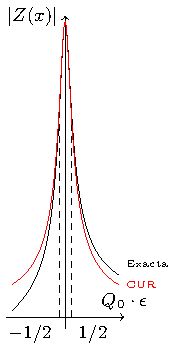
\includegraphics[height=0.8\textheight]{../figs/CUR.pdf}
\end{center}
\end{column}
\end{columns}
\end{frame}

\begin{frame}[label={sec:org76fe0c2}]{Puntos de potencia mitad en la CUR}
\begin{columns}
\begin{column}{0.7\columnwidth}
\begin{itemize}
\item La Curva Universal de Resonancia es simétrica: la frecuencia de resonancia está en el centro del ancho de banda.
\item Retomamos la expresión aproximada de los puntos de potencia mitad:
\end{itemize}
\[
  \omega_{1,2} \simeq \omega_0 (1 \mp \frac{1}{2Q_0})
\]
\end{column}

\begin{column}{0.3\columnwidth}
\begin{center}
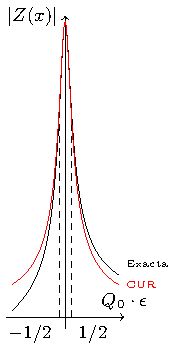
\includegraphics[height=0.7\textheight]{../figs/CUR.pdf}
\end{center}
\end{column}
\end{columns}

\begin{itemize}
\item Reescribimos usando la desintonización relativa:
\end{itemize}
\[
  \frac{\omega_{1,2} - \omega_0}{\omega_0} \simeq \mp \frac{1}{2Q_0}
\]

\[
  \boxed{x_{1,2} = Q_0 \cdot \epsilon_{1,2} = \mp \frac{1}{2}} \rightarrow Z(x_{1,2}) = \frac{1}{\sqrt{2}}
\]
\end{frame}

\section{Circuito RLC serie}
\label{sec:org80279ed}
\begin{frame}[label={sec:org33ebc56}]{Impedancia}
\begin{itemize}
\item Impedancia
\end{itemize}
\[
  \fasor{Z} = R + j(\omega L - \frac{1}{\omega C})
\]
\begin{itemize}
\item Impedancia en función de \(\omega_0\) y \(Q_0\)
\end{itemize}
\[
  \fasor{Z} = R \left[1 + j Q_0 \left(\frac{\omega}{\omega_0} - \frac{\omega_0}{\omega}\right)\right]
\]

\begin{itemize}
\item Impedancia en función de la desintonización relativa
\end{itemize}
\[
  \fasor{Z} = Z_0 \left[ 1 + j Q_0 \epsilon\left(\frac{2 + \epsilon}{1 + \epsilon}\right)\right]
\]  
\end{frame}

\begin{frame}[label={sec:org062d863}]{Frecuencias}
\begin{itemize}
\item Pulsación de Resonancia
\end{itemize}
\[
  \omega_0 = \frac{1}{\sqrt{LC}}
\]
\begin{itemize}
\item Puntos de Potencia Mitad
\end{itemize}
\[
\omega_{1,2}= \mp \frac{R}{2L} + \sqrt{\left(\frac{R}{2L}\right)^2 + \frac{1}{LC}}
\]

\begin{itemize}
\item Ancho de Banda
\end{itemize}
\[
B = \omega_2 - \omega_1 = \frac{R}{L}
\]

\begin{itemize}
\item Factor de Calidad
\end{itemize}
\[
  Q_0 = \frac{1}{\omega_0 C R} = \frac{\omega_0 L}{R}
\]
\end{frame}

\begin{frame}[label={sec:org4ddd5fd}]{Tensiones y energías}
\begin{itemize}
\item Tensiones en los elementos
\end{itemize}

\begin{align*}
  U(\omega_0) &= U_R(\omega_0)\\
  U_L(\omega_0) &= U_C(\omega_0) = Q_0 U
\end{align*}

\begin{itemize}
\item Energías almacenadas
\end{itemize}

\begin{align*}
  w_L(t) + w_c(t) &= \frac{1}{2} L I_0^2\\
  P_R &= R I^2\\
  w_{total} &= \frac{Q_0}{2\pi} w_R
\end{align*}
\end{frame}

\begin{frame}[label={sec:orgb8ea4ee}]{Curva Universal de Resonancia}
\begin{itemize}
\item Aproximación para cercanías de la resonancia
\end{itemize}
\[
  \fasor{Z} \simeq Z_0 (1 + j 2 Q_0 \epsilon)
\]

\[
  |\fasor{Z}| \simeq Z_0 \sqrt{1 + 4 Q^2_0 \epsilon^2}
\]
\begin{itemize}
\item Curva Universal de Resonancia
\end{itemize}
\[
  Y(x) = \frac{1}{\sqrt{1 + 4 x^2}}
\]
\end{frame}
\section{Otros circuitos}
\label{sec:org099560b}

\begin{frame}[label={sec:orgcde490c}]{Circuito RLC con bobina real}
\begin{center}
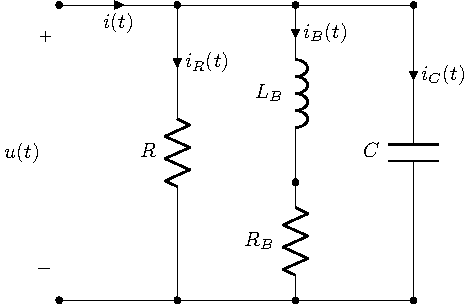
\includegraphics[height=0.4\textheight]{../figs/resonante_real.pdf}
\end{center}

La figura representa un circuito paralelo con una bobina real (con pérdidas). La impedancia de este circuito es:
\begin{align*}
\fasor{Y} &= \frac{1}{R} + j \omega C + \frac{1}{R_B + j \omega L_B} = \\ 
          &= \left(\frac{1}{R} + \frac{R_B}{R_B^2 + \omega^2 L_B^2}\right) + j \left(\omega C - \frac{\omega L_B}{R_B^2 + \omega^2 L_B^2}\right)
\end{align*}
\end{frame}

\begin{frame}[label={sec:org72e119a}]{Impedancia}
\[
\fasor{Y} = \left(\frac{1}{R} + \frac{R_B}{R_B^2 + \omega^2 L_B^2}\right) + j \left(\omega C - \frac{\omega L_B}{R_B^2 + \omega^2 L_B^2}\right)
\]
\begin{itemize}
\item Condición de Resonancia
\end{itemize}
\[
  \omega C - \frac{\omega L_B}{R_B^2 + \omega^2 L_B^2} = 0 
\]

\begin{itemize}
\item Pulsación de Resonancia
\end{itemize}
\[
\omega_0 = \sqrt{\frac{1}{L_BC} - \left(\frac{R_B}{L_B}\right)^2}
\]
\end{frame}
\begin{frame}[label={sec:orgecb343d}]{Comparación con RLC paralelo}
\begin{itemize}
\item La frecuencia de resonancia es diferente a un RLC serie/paralelo:
\end{itemize}

\[
\omega_0 \neq \frac{1}{\sqrt{LC}}
\]

\begin{itemize}
\item El valor máximo de la admitancia \alert{no} se alcanza en la frecuencia de resonancia, \(\omega_{max} \neq \omega_0\).

\item Cuando la \alert{bobina} tiene \alert{bajas pérdidas (Q alto)}, el circuito puede simplificarse a un RLC paralelo.
\end{itemize}
\end{frame}
\section{Factor de Calidad de Componentes}
\label{sec:org8657ef0}
\begin{frame}[label={sec:org00ca85a}]{Factor de Calidad}
\begin{itemize}
\item Retomamos la definición del factor de calidad como ratio entre la \alert{máxima energía almacenada} y la \alert{energía disipada en un período}.
\end{itemize}

\[
  Q(\omega) = 2\pi \frac{\max\{w_x(t)\}}{T \cdot P_R}
\]
\end{frame}

\begin{frame}[label={sec:org4fe2d1c}]{Bobina Real}
\begin{itemize}
\item Una bobina real tiene pérdidas resistivas debidas al hilo conductor\footnote{En algunos textos se emplea la tangente de pérdidas para caracterizar a la bobina real, siendo \(\tan{\delta} = 1/Q\).}.
\item Se modela como una conexión serie de una bobina ideal y una resistencia.
\end{itemize}
\begin{center}
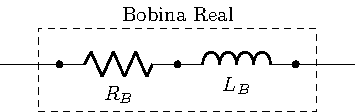
\includegraphics[height=0.2\textheight]{../figs/BobinaReal.pdf}
\end{center}

\[
  \left.
  \begin{array}{l}
    \max\{w_L(t)\} = \frac{1}{2} L_B I_o^2 = L_BI^2\\
      p_R(t) = R_B I^2
  \end{array}
  \right\} \rightarrow
  \boxed{Q(\omega) = \frac{\omega L_B}{R_B}}
\]
\end{frame}
\begin{frame}[label={sec:orgeaa7964}]{Condensador Real}
\begin{center}
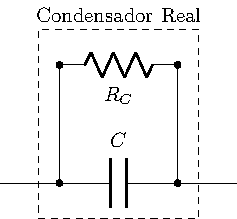
\includegraphics[height=0.5\textheight]{../figs/CondensadorReal.pdf}
\end{center}

\[
  \left.
  \begin{array}{l}
    \max\{w_C(t)\} = \frac{1}{2} C U_o^2 = CU^2\\
      p_R(t) = G_C U^2
  \end{array}
  \right\} \rightarrow
  \boxed{Q(\omega) = \omega C R_C}
\]
\end{frame}
\begin{frame}[label={sec:org83db95f}]{Ejercicio}
Demuestra que la expresión del factor de calidad de una bobina con pérdidas modelada como un circuito paralelo es:
\begin{columns}
\begin{column}{0.3\columnwidth}
\[
\boxed{Q = \frac{R_B}{\omega L_B}}
\]
\end{column}
\begin{column}{0.7\columnwidth}
\begin{center}
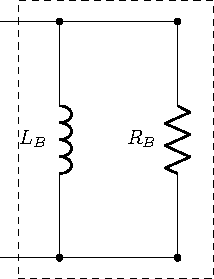
\includegraphics[height=0.7\textheight]{../figs/BobinaRealParalelo.pdf}
\end{center}
\end{column}
\end{columns}
\end{frame}


\begin{frame}[label={sec:orgfd02f48}]{Conversión serie-paralelo}
\begin{columns}
\begin{column}[t]{0.5\columnwidth}
\[
  \fasor{Y_s} = \frac{R_s - j\omega L_s}{R_s^2 + (\omega L_s)^2}
\]
\begin{center}
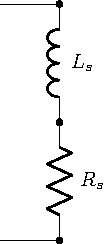
\includegraphics[height=0.4\textheight]{../figs/BobinaSerie.pdf}
\end{center}
\end{column}

\begin{column}[t]{0.5\columnwidth}
\[
  \fasor{Y_p} = \frac{1}{R_p} - j\frac{1}{\omega L_p}
\]
\begin{center}
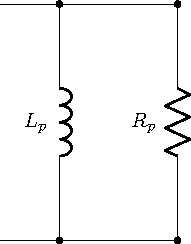
\includegraphics[height=0.4\textheight]{../figs/BobinaParalelo.pdf}
\end{center}
\end{column}
\end{columns}


\[
\left.
\begin{array}{l}
  R_p = \frac{R_s^2 + (\omega L_s)^2}{R_s}\\
  \omega L_p = \frac{R_s^2 + (\omega L_s)^2}{\omega L_s}
\end{array}
\right\} \Rightarrow
\frac{\omega L_s}{R_s} = \frac{R_p}{\omega L_p} \Rightarrow \boxed{Q_p = Q_s}
\]
\end{frame}

\begin{frame}[label={sec:org9164268}]{Conversión serie-paralelo}
\[
  \begin{array}{l}
      R_p = R_s + \frac{(\omega L_s)^2}{R_s} \xrightarrow{\omega L_s= Q_s \cdot R_s} \boxed{R_p = R_s ( 1 + Q_S^2)}\\
      \omega L_p = \omega L_s + \frac{R_s^2}{\omega L_s} \xrightarrow{R_s = \omega L_s/Q_s} \boxed{L_p = L_s (1 + 1/Q_s^2)}
  \end{array}
\]

Para bobinas con alto factor de calidad (\(Q \geq 10\))

\begin{columns}
\begin{column}{0.3\columnwidth}
\begin{center}
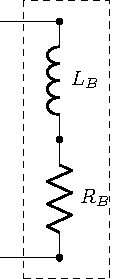
\includegraphics[height=0.4\textheight]{../figs/BobinaReal2.pdf}
\end{center}
\end{column}

\begin{column}{0.3\columnwidth}
\[
\boxed{
\begin{array}{l}
  R_p \simeq Q^2 \cdot R_s\\
  L_p \simeq L_s
\end{array}}
\]
\end{column}

\begin{column}{0.3\columnwidth}
\begin{center}
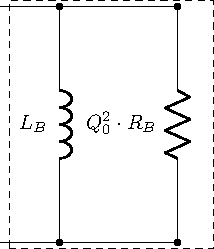
\includegraphics[height=0.4\textheight]{../figs/RL_paralelo.pdf}
\end{center}
\end{column}
\end{columns}
\end{frame}

\begin{frame}[label={sec:orgc863896}]{Conversión Serie-Paralelo}
Empleando ecuaciones similares se puede demostrar la siguiente transformación para un condensador de alto factor de calidad:
\begin{columns}
\begin{column}{0.3\columnwidth}
\begin{center}
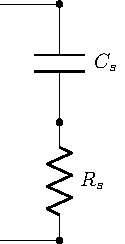
\includegraphics[height=0.4\textheight]{../figs/CondensadorSerie.pdf}
\end{center}
\end{column}
\begin{column}{0.3\columnwidth}
\[
\boxed{
\begin{array}{l}
  R_p \simeq Q^2 \cdot R_s\\
  C_p \simeq C_s
\end{array}}
\]
\end{column}

\begin{column}{0.3\columnwidth}
\begin{center}
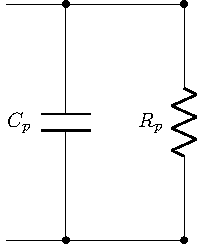
\includegraphics[height=0.4\textheight]{../figs/CondensadorParalelo.pdf}
\end{center}
\end{column}
\end{columns}
\end{frame}

\begin{frame}[label={sec:orgf342f71}]{Aplicación: transformación de circuito RLC}
\begin{center}
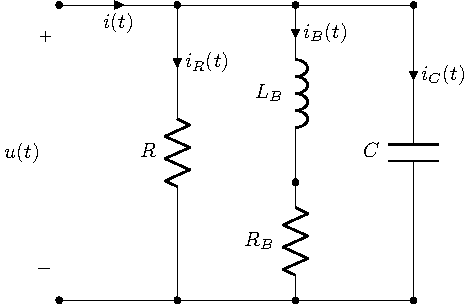
\includegraphics[height=0.8\textheight]{../figs/resonante_real.pdf}
\end{center}
\end{frame}

\begin{frame}[label={sec:orgde4e7ab}]{Ejercicios Recomendados}
\begin{itemize}
\item AS: ejemplos 14.7 y 14.8
\item HKD: página 641 (voltímetro), y práctica 16.8
\item PO: problemas 23.5 y 23.7
\end{itemize}
\end{frame}
\end{document}